\documentclass[12pt]{rapportECL}
\usepackage{lipsum}
\usepackage{fancybox}
\usepackage{float}
\usepackage{amsbsy}
\usepackage{amssymb}
\usepackage{listings}
\lstset{breaklines=true}
\usepackage{stmaryrd}
\usepackage{pdfpages}
\title{rapport\_tp1} %Titre du fichier
\renewcommand{\thesection}{\arabic{section}} 
\newcommand{\fact}[1]{#1\mathpunct{}!}

\begin{document}

%----------- Informations du rapport ---------

\titre{Modélisation des données} %Titre du fichier .pdf
%\UE{UE PRO} %Nom de la UE
%\sujet{\LaTeX Approfondi} %Nom du sujet

\enseignant{
	Renaud \textsc{Vérin}
} %Nom de l'enseignant

\eleves{
	\textsc{BURIE} Aurélien \\
	\textsc{LAFAGE} Adrien \\
	\textsc{LEROUX} Louis-Clément \\
	\textsc{PARAU} Emmanuel
} %Nom des élèves

%----------- Initialisation -------------------
        
\fairemarges %Affiche les marges
\fairepagedegarde %Crée la page de garde
\setcounter{page}{1}

%------------ Corps du rapport ----------------

\section{Introduction}

L'objectif de ce rapport est de vous présenter la façon dont nous avons modlisé les données fournies par le client VDSA. En effet, on nous a fourni un tableau contenant l'ensemble des données concernant les clients de l'entreprise. Nous avons donc créé pour cela plusieurs entités dont les relations vous seront explicités par le biais d'un modèle conceptuel et d'un modèle logique de nos données. Finalement, vous trouverez le code SQL correspondant. 

\tabledematieres %Crée la table des matières
\section{Modèle conceptuel}

Les données fournies sont de la forme suivante : \\
\begin{figure}[h]
	\begin{center}
		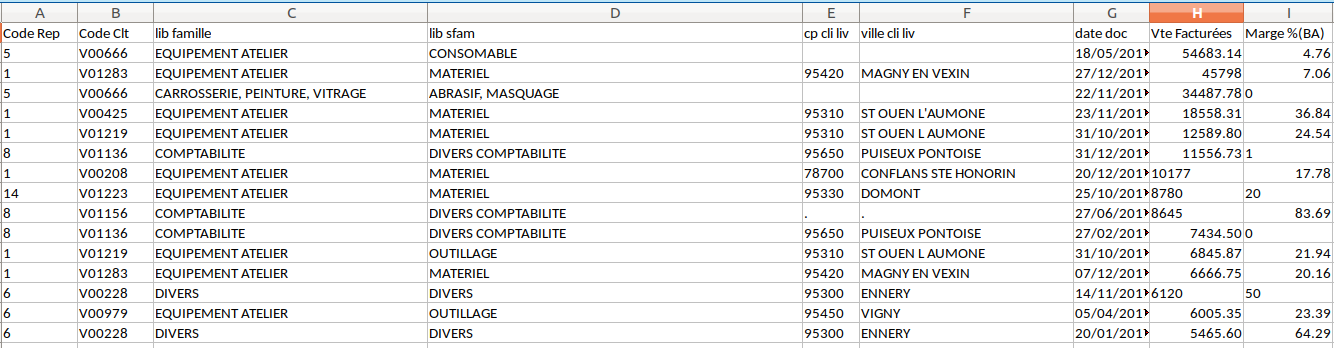
\includegraphics[scale=0.35]{img/data.png}
		\caption{Exemple de données fournies par VDSA}
	\end{center}
\end{figure}

De celles-ci nous en avons déduis les entités : Client, Commande, Article, Famille, Sous-Famille.
Un client possède un code (Code Clt), une adresse, un code postal (cp cli liv) et une ville (ville cli liv). Une commande est composée d'un identifiant, d'une date (date doc), d'un lieu, d'une marge (Marge\%(BA)) et d'un chiffre d'affaire. Un article a un identifiant et une date d'achat. Une famille possède une code pour l'identifer et d'un libellé (lib famille). Une sous-famille comprend un code pour l'identifier et d'un libellé (lib sfam).\\
De plus, notre site devra gérer des comptes utilisateur. Ainsi nous avons en plus créé l'entité Utilisateur. Celle-ci est constituée d'un identifiant, d'un nom, d'un prénom, d'un mail et d'un mot de passe. L'utilisateur pourra avoir un rôle qui lui est associé (exemple : administrateur). Soit le rôle fera parti de l'entité Utilisateur, soit nous créerons l'entité Rôle. Celle-ci sera composée d'un identifiant et d'un nom.\\ \\
\noindent
Vous trouverez sur la page suivante le modèle conceptuel de nos données.

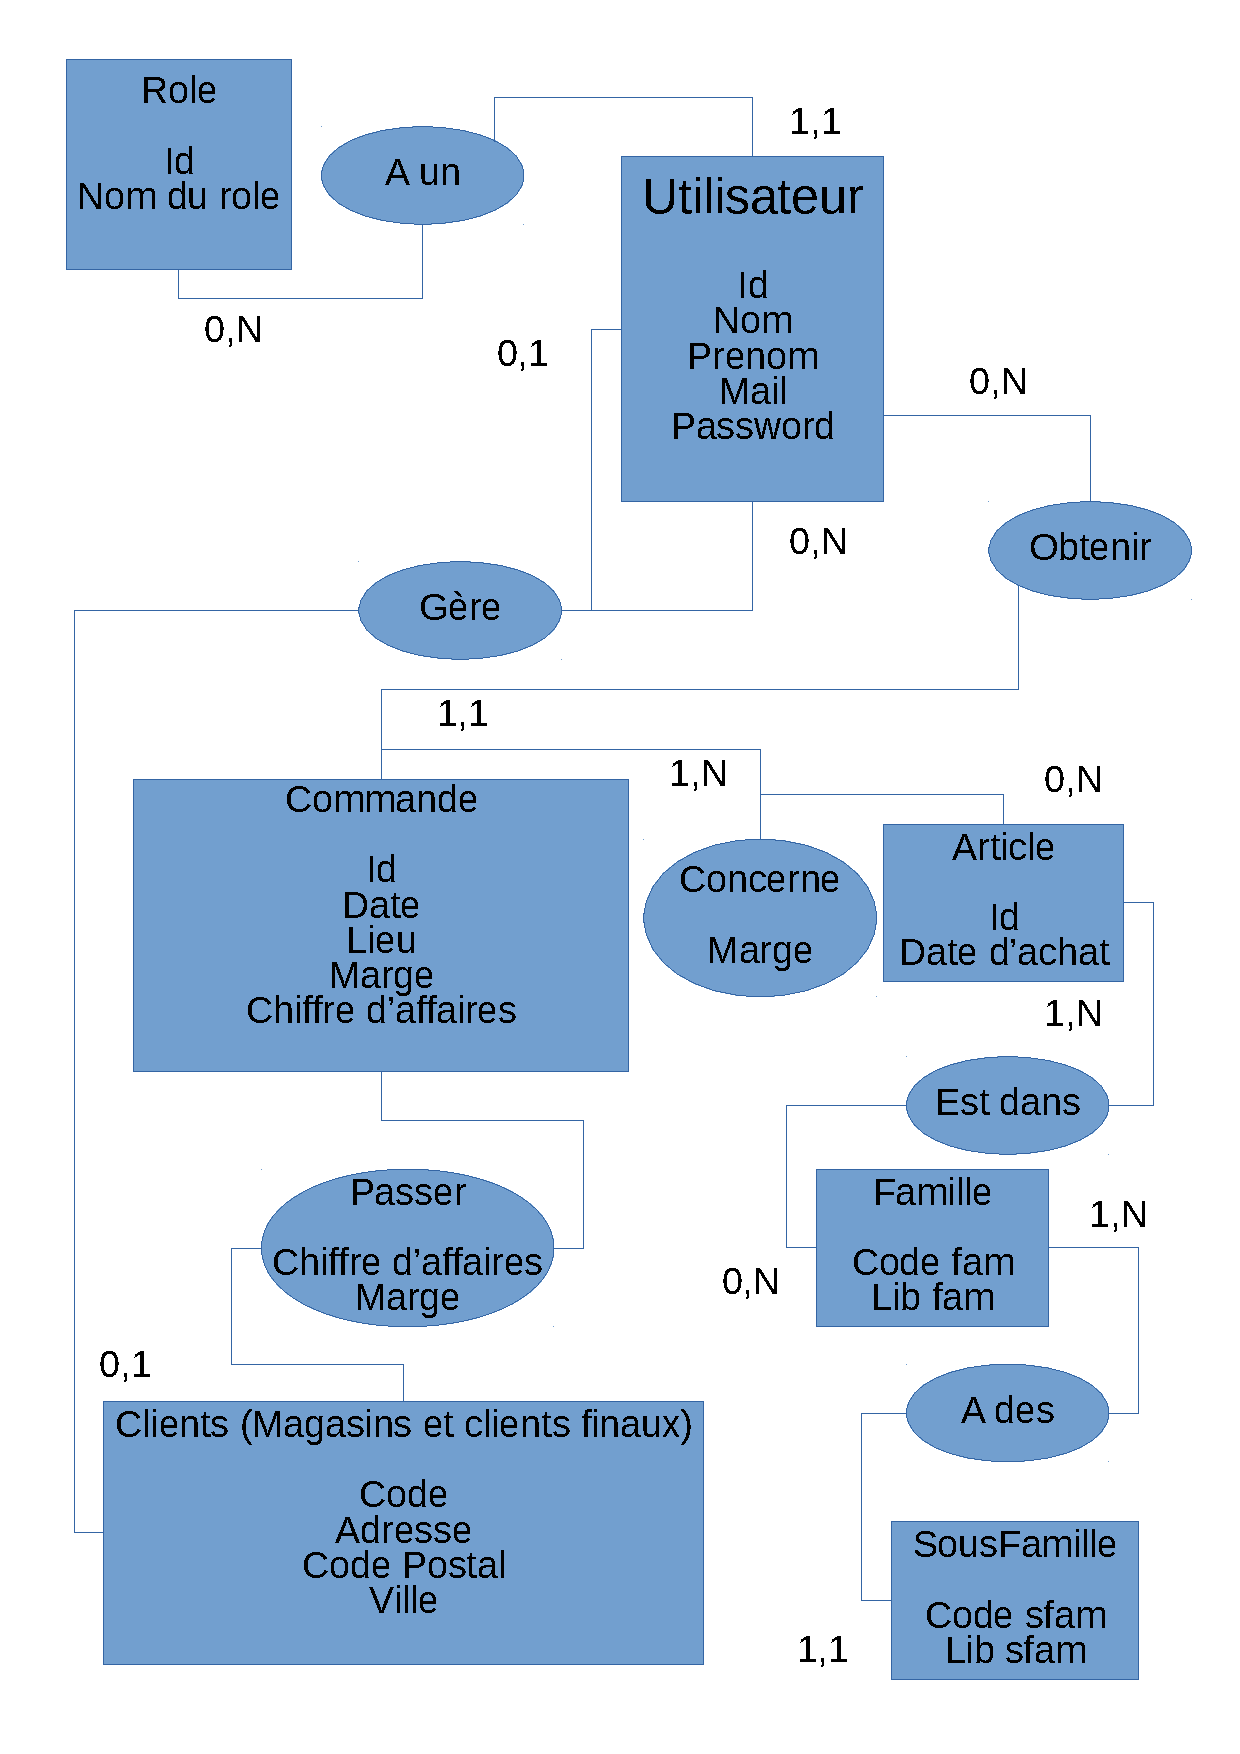
\includepdf{mcd.pdf}
\clearpage
\section{Modèle logique}

En utilisant le modèle conceptuel de nos données nous en déduisons le modèle logique suivant :
\begin{enumerate}
\item[•] Utilisateur(\underline{id}, nom, prenom, mail, password, role*)
\item[•] Client(\underline{code}, code postal, ville, \#id\_utilisateur)
\item[•] Commande(\underline{id}, date, code Postal, ville, margeTotal, chiffre\_affaires, \#id\_utilisateur)
\item[•] Composition(\underline{\#id\_commande, \#id\_article}, marge)
\item[•] Article(\underline{id}, dateAchat, \#codeFam\_famille)
\item[•] Famille(\underline{codeFam}, libFam)
\item[•] SousFamille(\underline{codeSfam}, libSfam, \#codeFam\_famille) \\
\end{enumerate}


\clearpage
\section{Code source SQL}

Voici comment nous créons nos entités en SQL :
\begin{enumerate}
\item[•] Utilisateur : \\
\lstinputlisting[language=SQL, firstline=1, lastline=10]{source.sql}
\item[•] Client : \\
\lstinputlisting[language=SQL, firstline=21, lastline=29]{source.sql}
\item[•] Commande : \\
\lstinputlisting[language=SQL, firstline=31, lastline=40]{source.sql}
\item[•] Famille : \\
\lstinputlisting[language=SQL, firstline=42, lastline=46]{source.sql}
\item[•] Sous-Famille : \\
\lstinputlisting[language=SQL, firstline=48, lastline=54]{source.sql}
\item[•] Article : \\
\lstinputlisting[language=SQL, firstline=56, lastline=62]{source.sql}
\item[•] Composition : \\
\lstinputlisting[language=SQL, firstline=64, lastline=71]{source.sql}
\end{enumerate}

\noindent
\textit{Si nous choisissons finalement de créer une entité Role, on aura :}\\
\lstinputlisting[language=SQL, firstline=12, lastline=18]{source.sql}

%------------ Fin du document  -----------------
\end{document}

%https://openclassrooms.com/forum/sujet/formulaire-de-formules-latex-84687
